%%%%%%%%%%%%%%%%%%%%%%%%%%%%%%%%%%%%%%%%%%%%%%%%%%%%%%%%%%%%%%%%%%%%%%%%
% Plantilla TFG/TFM
% Escuela Politécnica Superior de la Universidad de Alicante
% Realizado por: Jose Manuel Requena Plens
% Contacto: info@jmrplens.com / Telegram:@jmrplens
%%%%%%%%%%%%%%%%%%%%%%%%%%%%%%%%%%%%%%%%%%%%%%%%%%%%%%%%%%%%%%%%%%%%%%%%

\chapter{Anexo I}
\label{anexos}

\section{Anexo 1}
\subsection{Gráficas del cálculo de distancias del modelo 1}
\begin{figure}[H]
	\centering
	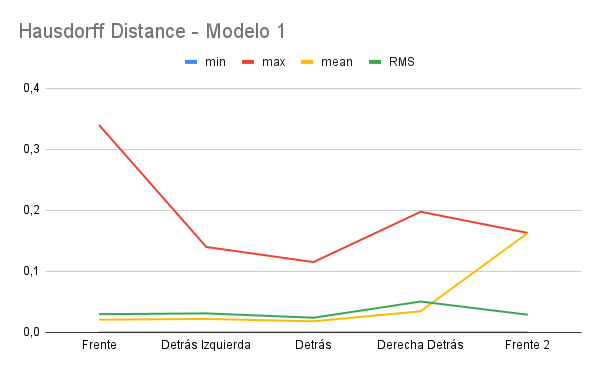
\includegraphics[scale=0.55]{imagenes/Hausdorff-M1.png}
	\caption{Gráfica sobre los cálculos obtenidos con Hausdorff y el modelo 1 comparado con los modelos en diferentes ángulos obtenidos con la red PIFu[\cite{pifu}]}
	\label{fig:figura14}
\end{figure}

\begin{figure}[H]
	\centering
	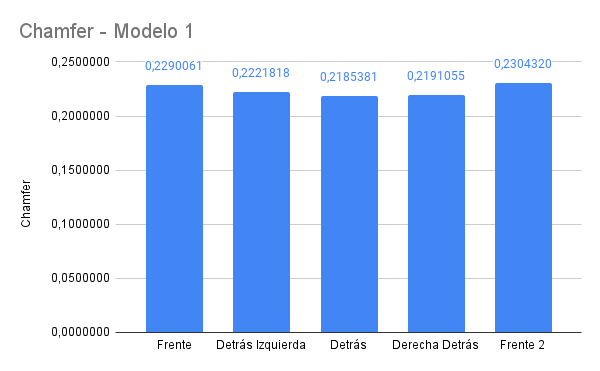
\includegraphics[scale=0.55]{imagenes/Chamfer-M1.png}
	\caption{Gráfica sobre los cálculos obtenidos con Chamfer y el modelo 1 comparado con los modelos en diferentes ángulos obtenidos con la red PIFu[\cite{pifu}]}
	\label{fig:figura15}
\end{figure}
\subsection{Gráficas del cálculo de distancias del modelo 2}
\begin{figure}[H]
	\centering
	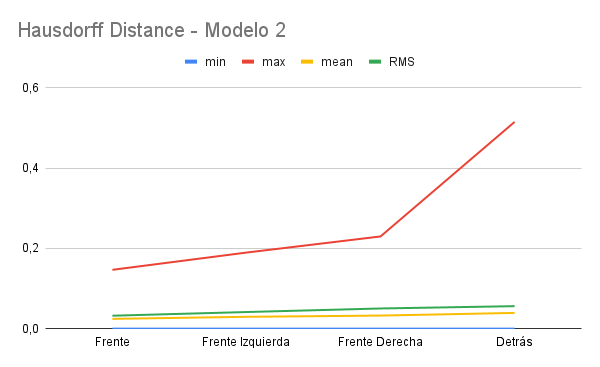
\includegraphics[scale=0.55]{imagenes/Hausdorff-M2.png}
	\caption{Gráfica sobre los cálculos obtenidos con Hausdorff y el modelo 2 comparado con los modelos en diferentes ángulos obtenidos con la red PIFu[\cite{pifu}]}
	\label{fig:figura16}
\end{figure}

\begin{figure}[H]
	\centering
	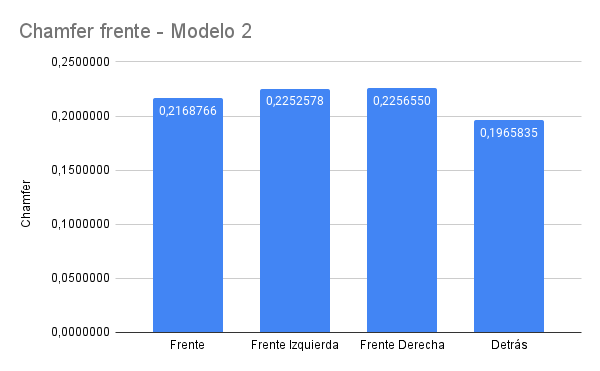
\includegraphics[scale=0.55]{imagenes/Chamfer-M2.png}
	\caption{Gráfica sobre los cálculos obtenidos con Chamfer y el modelo 2 comparado con los modelos en diferentes ángulos obtenidos con la red PIFu[\cite{pifu}]}
	\label{fig:figura17}
\end{figure}
\subsection{Gráficas del cálculo de distancias del modelo 3}
\begin{figure}[H]
	\centering
	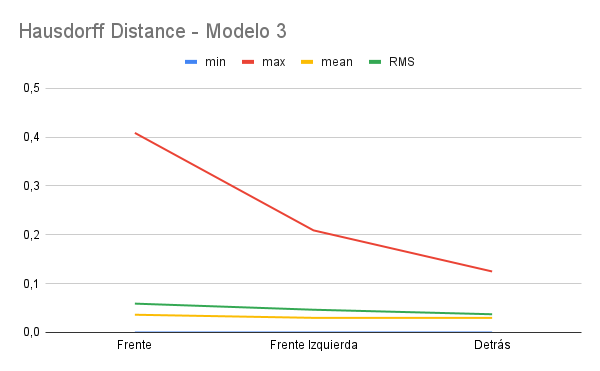
\includegraphics[scale=0.55]{imagenes/Hausdorff-M3.png}
	\caption{Gráfica sobre los cálculos obtenidos con Hausdorff y el modelo 3 comparado con los modelos en diferentes ángulos obtenidos con la red PIFu[\cite{pifu}]}
	\label{fig:figura18}
\end{figure}

\begin{figure}[H]
	\centering
	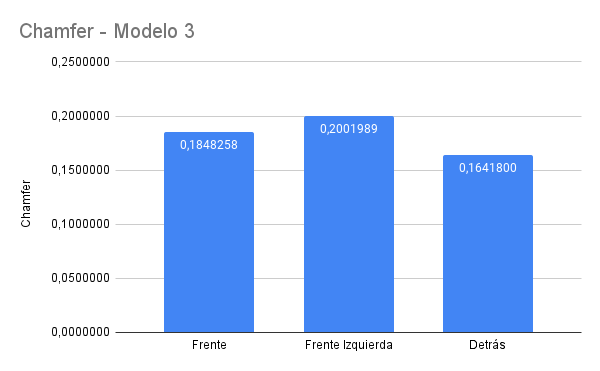
\includegraphics[scale=0.55]{imagenes/Chamfer-M3.png}
	\caption{Gráfica sobre los cálculos obtenidos con Chamfer y el modelo 3 comparado con los modelos en diferentes ángulos obtenidos con la red PIFu[\cite{pifu}]}
	\label{fig:figura19}
\end{figure}


\section{Anexo 2}

\subsection{Modelos con ruido añadido}

\begin{figure}[H]
	\centering
	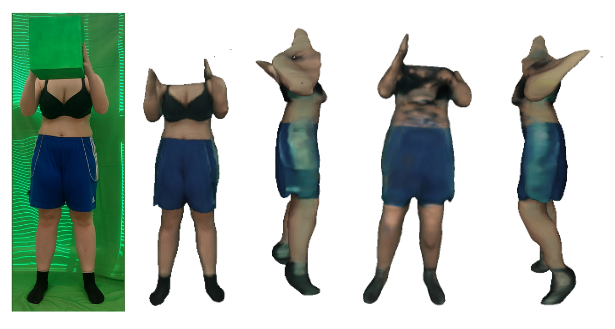
\includegraphics[scale=0.65]{imagenes/cameliae.png}
	\caption{Modelo obtenido con ruido en la cabeza}
	\label{fig:figura20}
\end{figure}

\begin{figure}[H]
	\centering
	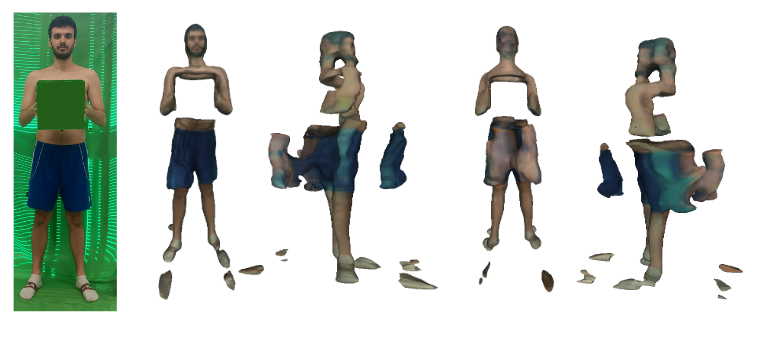
\includegraphics[scale=0.65]{imagenes/nahuele1.png}
	\caption{Modelo obtenido con ruido en el pecho}
	\label{fig:figura21}
\end{figure}

\begin{figure}[H]
	\centering
	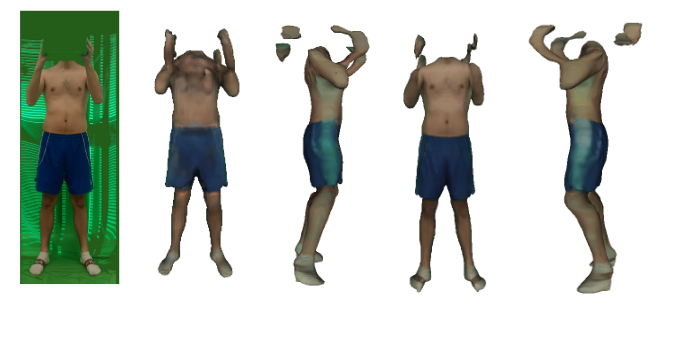
\includegraphics[scale=0.65]{imagenes/nahuele2.png}
	\caption{Modelo obtenido con ruido en la cabeza}
	\label{fig:figura22}
\end{figure}

\section{Anexo 3}

\subsection{Modelo 1}
\begin{figure}[H]
	\centering
	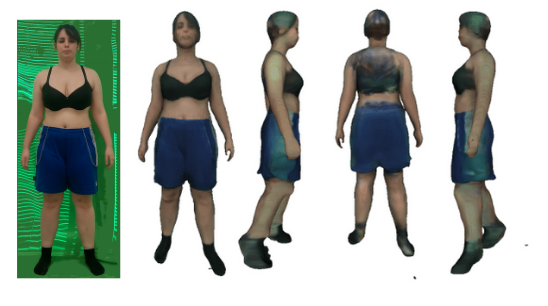
\includegraphics[scale=0.65]{imagenes/camelia0.png}
	\caption{Modelo 1, vista Frente}
	\label{fig:c1}
\end{figure}
\begin{figure}[H]
	\centering
	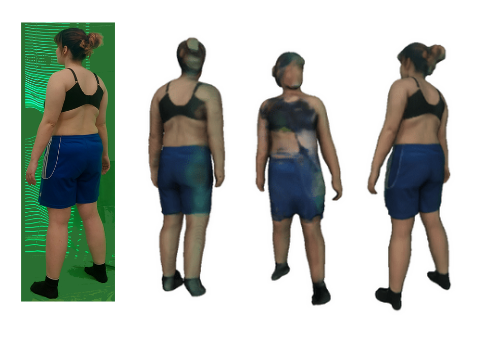
\includegraphics[scale=0.65]{imagenes/camelia5.png}
	\caption{Modelo 1, vista Detrás-Izquierda}
	\label{fig:c2}
\end{figure}
\begin{figure}[H]
	\centering
	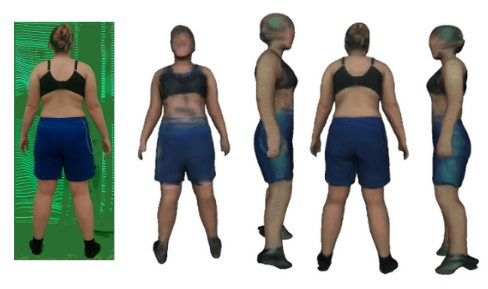
\includegraphics[scale=0.65]{imagenes/camelia6.png}
	\caption{Modelo 1, vista Detrás}
	\label{fig:c3}
\end{figure}
\begin{figure}[H]
	\centering
	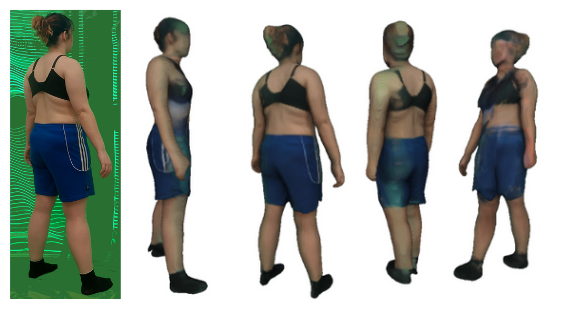
\includegraphics[scale=0.65]{imagenes/camelia7.png}
	\caption{Modelo 1, vista Detrás-Derecha}
	\label{fig:c4}
\end{figure}
\begin{figure}[H]
	\centering
	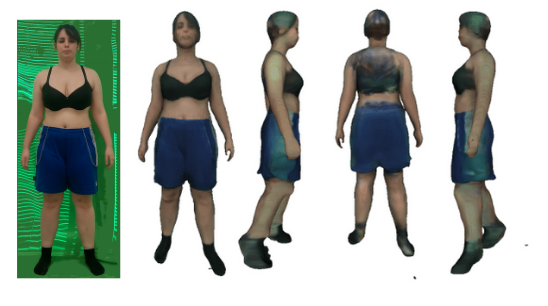
\includegraphics[scale=0.65]{imagenes/camelia0.png}
	\caption{Modelo 1, vista Frente 2}
	\label{fig:c5}
\end{figure}

\subsection{Modelo 2}
\begin{figure}[H]
	\centering
	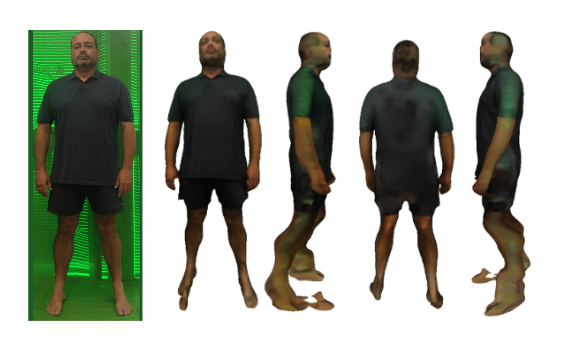
\includegraphics[scale=0.65]{imagenes/andres1.png}
	\caption{Modelo 2, vista Frente}
	\label{fig:a1}
\end{figure}
\begin{figure}[H]
	\centering
	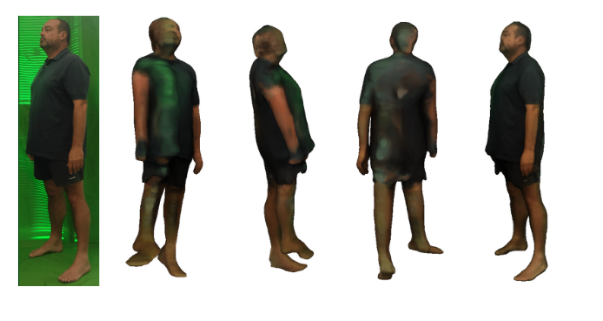
\includegraphics[scale=0.65]{imagenes/andres2.png}
	\caption{Modelo 2, vista Frente-Izquierda}
	\label{fig:a2}
\end{figure}
\begin{figure}[H]
	\centering
	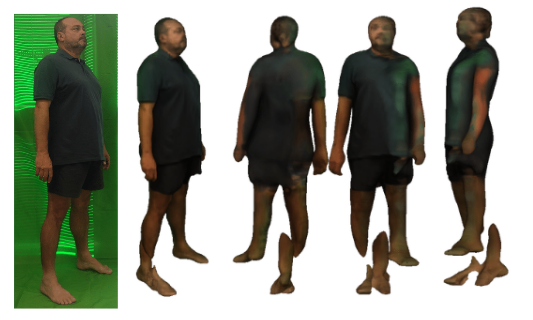
\includegraphics[scale=0.65]{imagenes/andres3.png}
	\caption{Modelo 2, vista Frente-Derecha}
	\label{fig:a3}
\end{figure}
\begin{figure}[H]
	\centering
	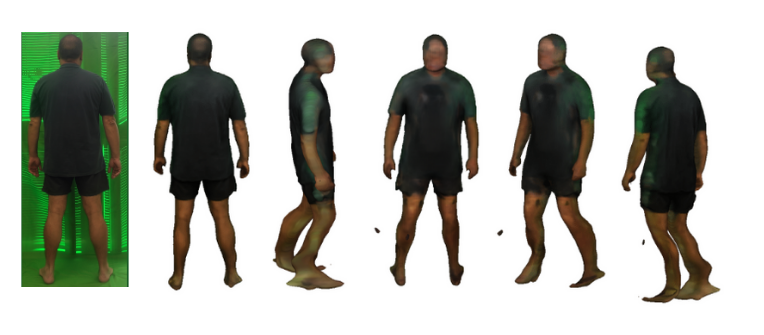
\includegraphics[scale=0.65]{imagenes/andres4.png}
	\caption{Modelo 2, vista Detrás}
	\label{fig:a4}
\end{figure}
\subsection{Modelo 3}

\begin{figure}[H]
	\centering
	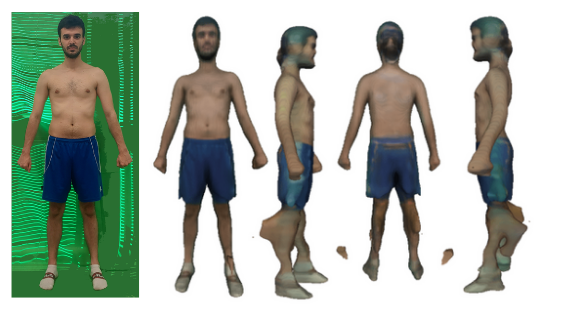
\includegraphics[scale=0.65]{imagenes/nahuel1.png}
	\caption{Modelo 3, vista Frente}
	\label{fig:n1}
\end{figure}
\begin{figure}[H]
	\centering
	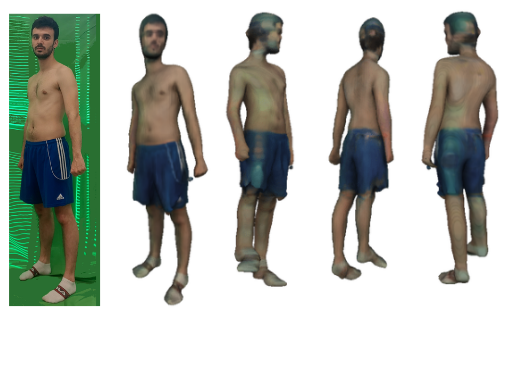
\includegraphics[scale=0.65]{imagenes/nahuel2.png}
	\caption{Modelo 3, vista Frente-Izquierda}
	\label{fig:n2}
\end{figure}
\begin{figure}[H]
	\centering
	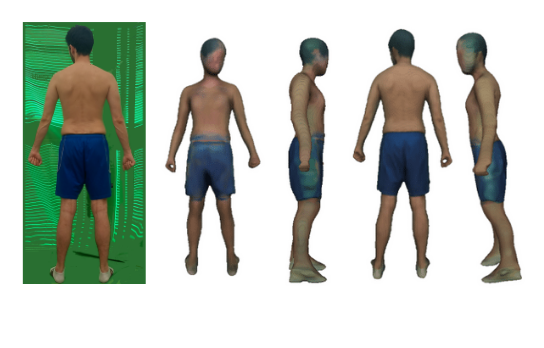
\includegraphics[scale=0.65]{imagenes/nahuel3.png}
	\caption{Modelo 3, vista Detrás}
	\label{fig:n3}
\end{figure}
